\chapter{Systemic Testing of Available Bacteria Speciation Models}

\begin{shadequote}
I wanna make sure you're ready, brother. Here it is: Show me the money. Oh-ho-ho! SHOW! ME! THE! MONEY! A-ha-ha! Jerry, doesn't it make you feel good just to say that! Say it with me one time, Jerry. \par\emph{Rod Tidwell}
\end{shadequote}


\section{Methods}
Most methods used were based on a previous study, with few modifications~\cite{carlo}.
Our main goals were to test ES2's accuracy for small input sizes, large input sizes, and show ES2's speed improvements over ES1.
This involves many \emph{in silico} or computer generated dataset tests, and a test of ES2 on previous \emph{Bacillus} data samples from Death Valley.

\begin{figure}[h!]
\centering
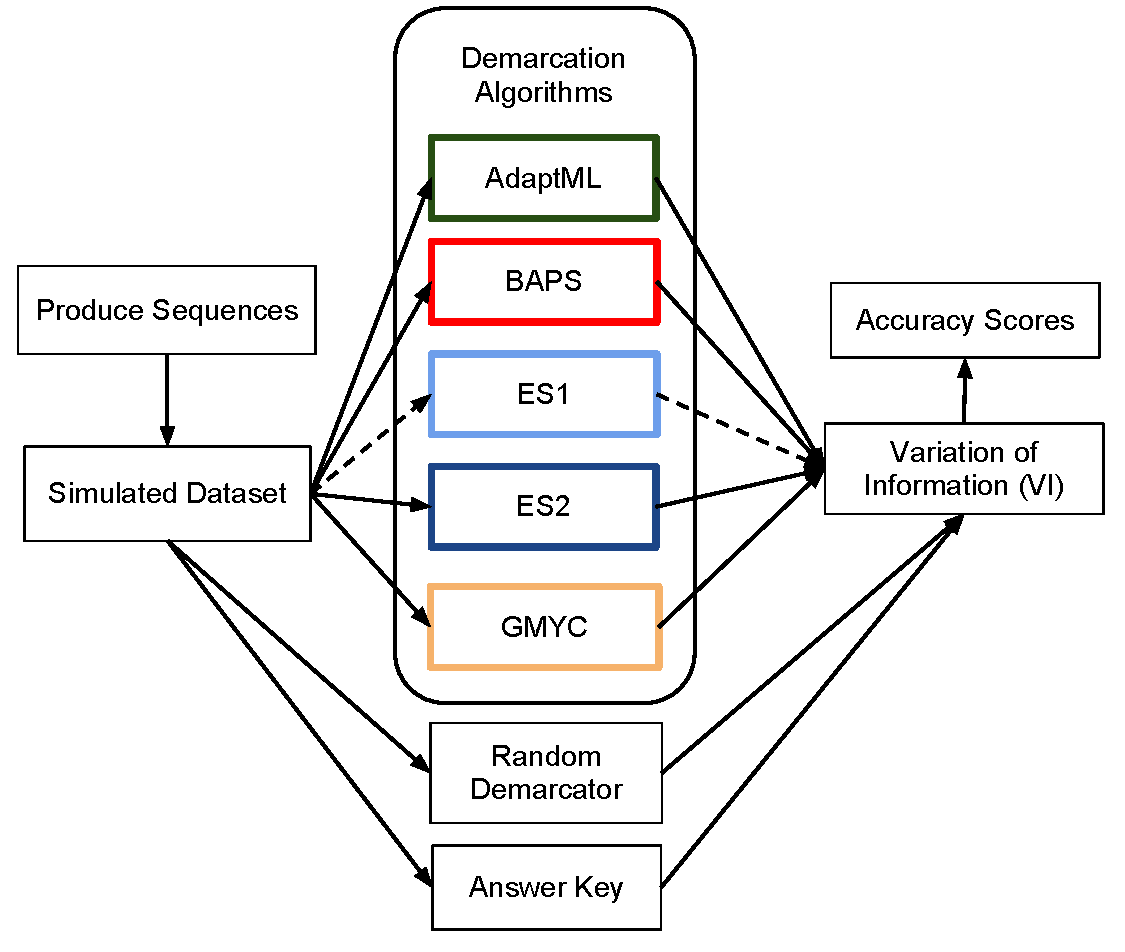
\includegraphics[scale=0.75]{images/DemarcationComparisonsFlow-CH4}
\caption[Demarcation comparison flow diagram.]{A flow diagram for the running of demarcation accuracy comparisons. The produce sequences makes simulated datasets that are used as inputs for various demarcation algorithms, the random demarcator, and answer key generation. All the resulting output is compared with the Variation of Information (VI) metric to determine accuracy. The dotted line is present because ES1 is not run on the larger datasets.}
\label{fig:ComparisonFlow}
\end{figure}

\subsection*{Other demarcation algorithms}
As a right of passage, we compare ES against other available demarcation algorithms~\cite{carlo}.
Previously, ES was demonstrated to be the most accurate, yet slowest demarcator.
ES2 aims to be just as accurate as ES but a lot faster, enabling larger input size functionality.
However, there are other demarcators currently available that utilize a variety of clustering models.

\subsubsection*{GMYC~\cite{barraclough2009inferring}}
The GMYC algorithm assumes a Yule model of speciation followed by a neutral coalescent model within species, where drift is the only process yielding coalescence.
It was originally designed to delineate species from sequences for sexually reproducing organisms such as insects, but later was shown to be applicable to asexually reproducing organisms.
GMYC needs only an ultrametric phylogentic tree to demarcate strains.
It is available as a part of the SPLITS package installed and imported onto any local R environment on Mac, Linux, and Windows.

\subsubsection*{BAPS~\cite{corander2007bayesian}}
The Bayesian Analysis of Population Structure (BAPS) application refines existing Bayesian approaches to determine the structure of populations from genetic data.
It assumes a partition-based mixture model and performs classification using a variant of the Metropolis-Hasting algorithm to identify clusters of sequences, with no explicit model of purging diversity within clusters.
Although, the algorithm can take into account recombination within and between populations.

BAPS has Windows, Linux and Mac versions with GUIs and a command line interface designed for batch processing, however it does not function in the Mac platform.

\subsubsection*{AdaptML~\cite{hunt2008resource}}
AdaptML places strains into ecotypes based on the assumption that the origin of each ecotype is driven by a change in habitat preferences.
Unlike the cohesion-based algorithms, it only requires a phylogentic tree and data specifying habitat isolation measurements for each strain.
The algorithm assumes a hidden Markov model for the evolution of habitat association and maximizes the likelihood of associations of the strains observed on the tree.

AdaptML runs on any operating system with a  version of Python installed. There is also a web app version of the algorithm where one can upload the data set and have AdaptML demarcations emailed.

\subsubsection*{Random demarcation}
I quickly developed a random demarcator to serve as a control. In it I pick a random number between one and the number of samples for $npop$, then I randomly distribute the generated sequences throughout $npop$ ecotypes.
[SEE CODE IN APPENDIX or FIGURE?]

\begin{figure}[h!]
\centering
\noindent\code{Random Demarcation}{code/random_formatted.py}
\caption[Python code showing a random demarcator.]{A description with more to be added soon, code needs to be cleaned up.}
\label{code:RandomDemarcating}
\end{figure}


\subsection*{Generation of sequences for analysis}
In order to compare the accuracy of several demarcation programs, the true parameters of the test data must be known.
The problem can be summarized as generating a history for a monophyletic group of $x$ organisms.
Clade history was based on an ecotype formation rate ($\Omega$), the rate of periodic selection ($\sigma$), and the number of ecotypes (\emph{npop}) within the sample.
We used the Ecotype Simulation algorithm to generate each organism's sequence and ecotype affiliation.
Habitats were indicated by either an ``A'' or ``B''.
We generated datasets with differing numbers of simulated sequences, and based them on three values each of $\Omega$, and $\sigma$.
The middle values of $\Omega$ and $\sigma$ were 0.19 and 1.1 respectively, based on prior ES simulation of \emph{Bacillus} in a Death Valley canyon.
Lower and upper values represented a difference of a factor of 10 of the \emph{Bacillus} values.
$Npop$ values were chosen based on the specific run's input size.
We generally tried to choose $npop$ values of 10, 30, and 40 percent regarding input size.

\subsubsection*{Preparing the input}
PhyML~\cite{guindon2010new}, a maximum likelihood tree construction algorithm, was used to build a phylogenetic tree from generated sequences.
The tree was converted into an ultra metric chronogram using Sanderson's nonparametric rate smoothing algorithm, which is included in the APE package.
This ultra metric tree was used as input for GMYC.

AdaptML requires the habitat from which each strain was isolated.
In previous studies we designed a specialization metric for designating habitats, however we found a specific unit of this metric that worked best~\cite{carlo}.
Thus, we will stick to using the best parameter of habitat specialization for AdaptML analysis.

FASTA sequences were converted into XLS format for compatibility with the BAPS package.

\subsection*{Variation of Information Metric}
The Variation of Information (VI) metric~\cite{meilua2003comparing} was used as a criterion for comparing two partitions of the same data set, to determine the closeness of each algorithm's ecotype demarcations to the canonical demarcations generated \emph{in silico}.
The Variation of Information between two clusterings C and C' is given by$$VI(C, C') = H(C) + H(C') - 2I(C, C')$$where H(C) is the entropy of a random variable associated with a sequence being in a cluster C and I(C,C') is the mutual information of the two associated variables.

\subsection*{ES2 on smaller datasets}
I ran the new and improved ES2 algorithm on generated datasets for parameters clearly defined in previous studies~\cite{carlo}.
All sample datasets included fifty sequences, and was repeated ten times to find the mean Variation of Information score.

On a few specific values we ran ES1 and ES2 through one hundred repetitions to find more robust VI scores.

\subsubsection*{Bacillus sequences}
\emph{Bacillus} strains were isolated from Radio Facility Wash, a west-running canyon in Death Valley, consisting of a habitats with three levels of solar exposure, including the canyon's sunny south-facing slope, the shadier and cooler north-facing slope, and the arroyo at the bottom.
Solar exposure habitats served as the only ecological dimension used for environmental input into AdaptML.
Sequence processing, was done as previously reported~\cite{carlo}.
Again we used PhyML to produce a maximum likelihood tree.

\subsection*{All demarcation programs on large datasets}
We ran all demarcations programs, and a random demarcator on generated datasets of 100, 200, 400 and X sequences.
Parameters were once again adopted from previous studies.
The exception being a choice of $npop$ which, was [rational for npop choices].

\subsection*{Running Time Tests}
We tested the running time of each algorithm on a [computer details].
We present the mean run times that each algorithm required to analyze synthetic data sets constructed using the parameter values estimated previously for \emph{Bacillus}, with [give speed run details].

\section{Results and Discussion}

%Proof of concept for a figure!
\begin{figure}[h!]
  \caption[Demarcation comparison table for small inputs (nu = 50).]{A comparison table of all demarcation algorithms run with differing sigma, omega, and npop values on input sizes of 50 sequences. Parameter combinations in which ES2 outperformed ES1 are circled in red. [I probably won't put in the full table, but parts of it and leave the big one for the appendix]}
  \centering
    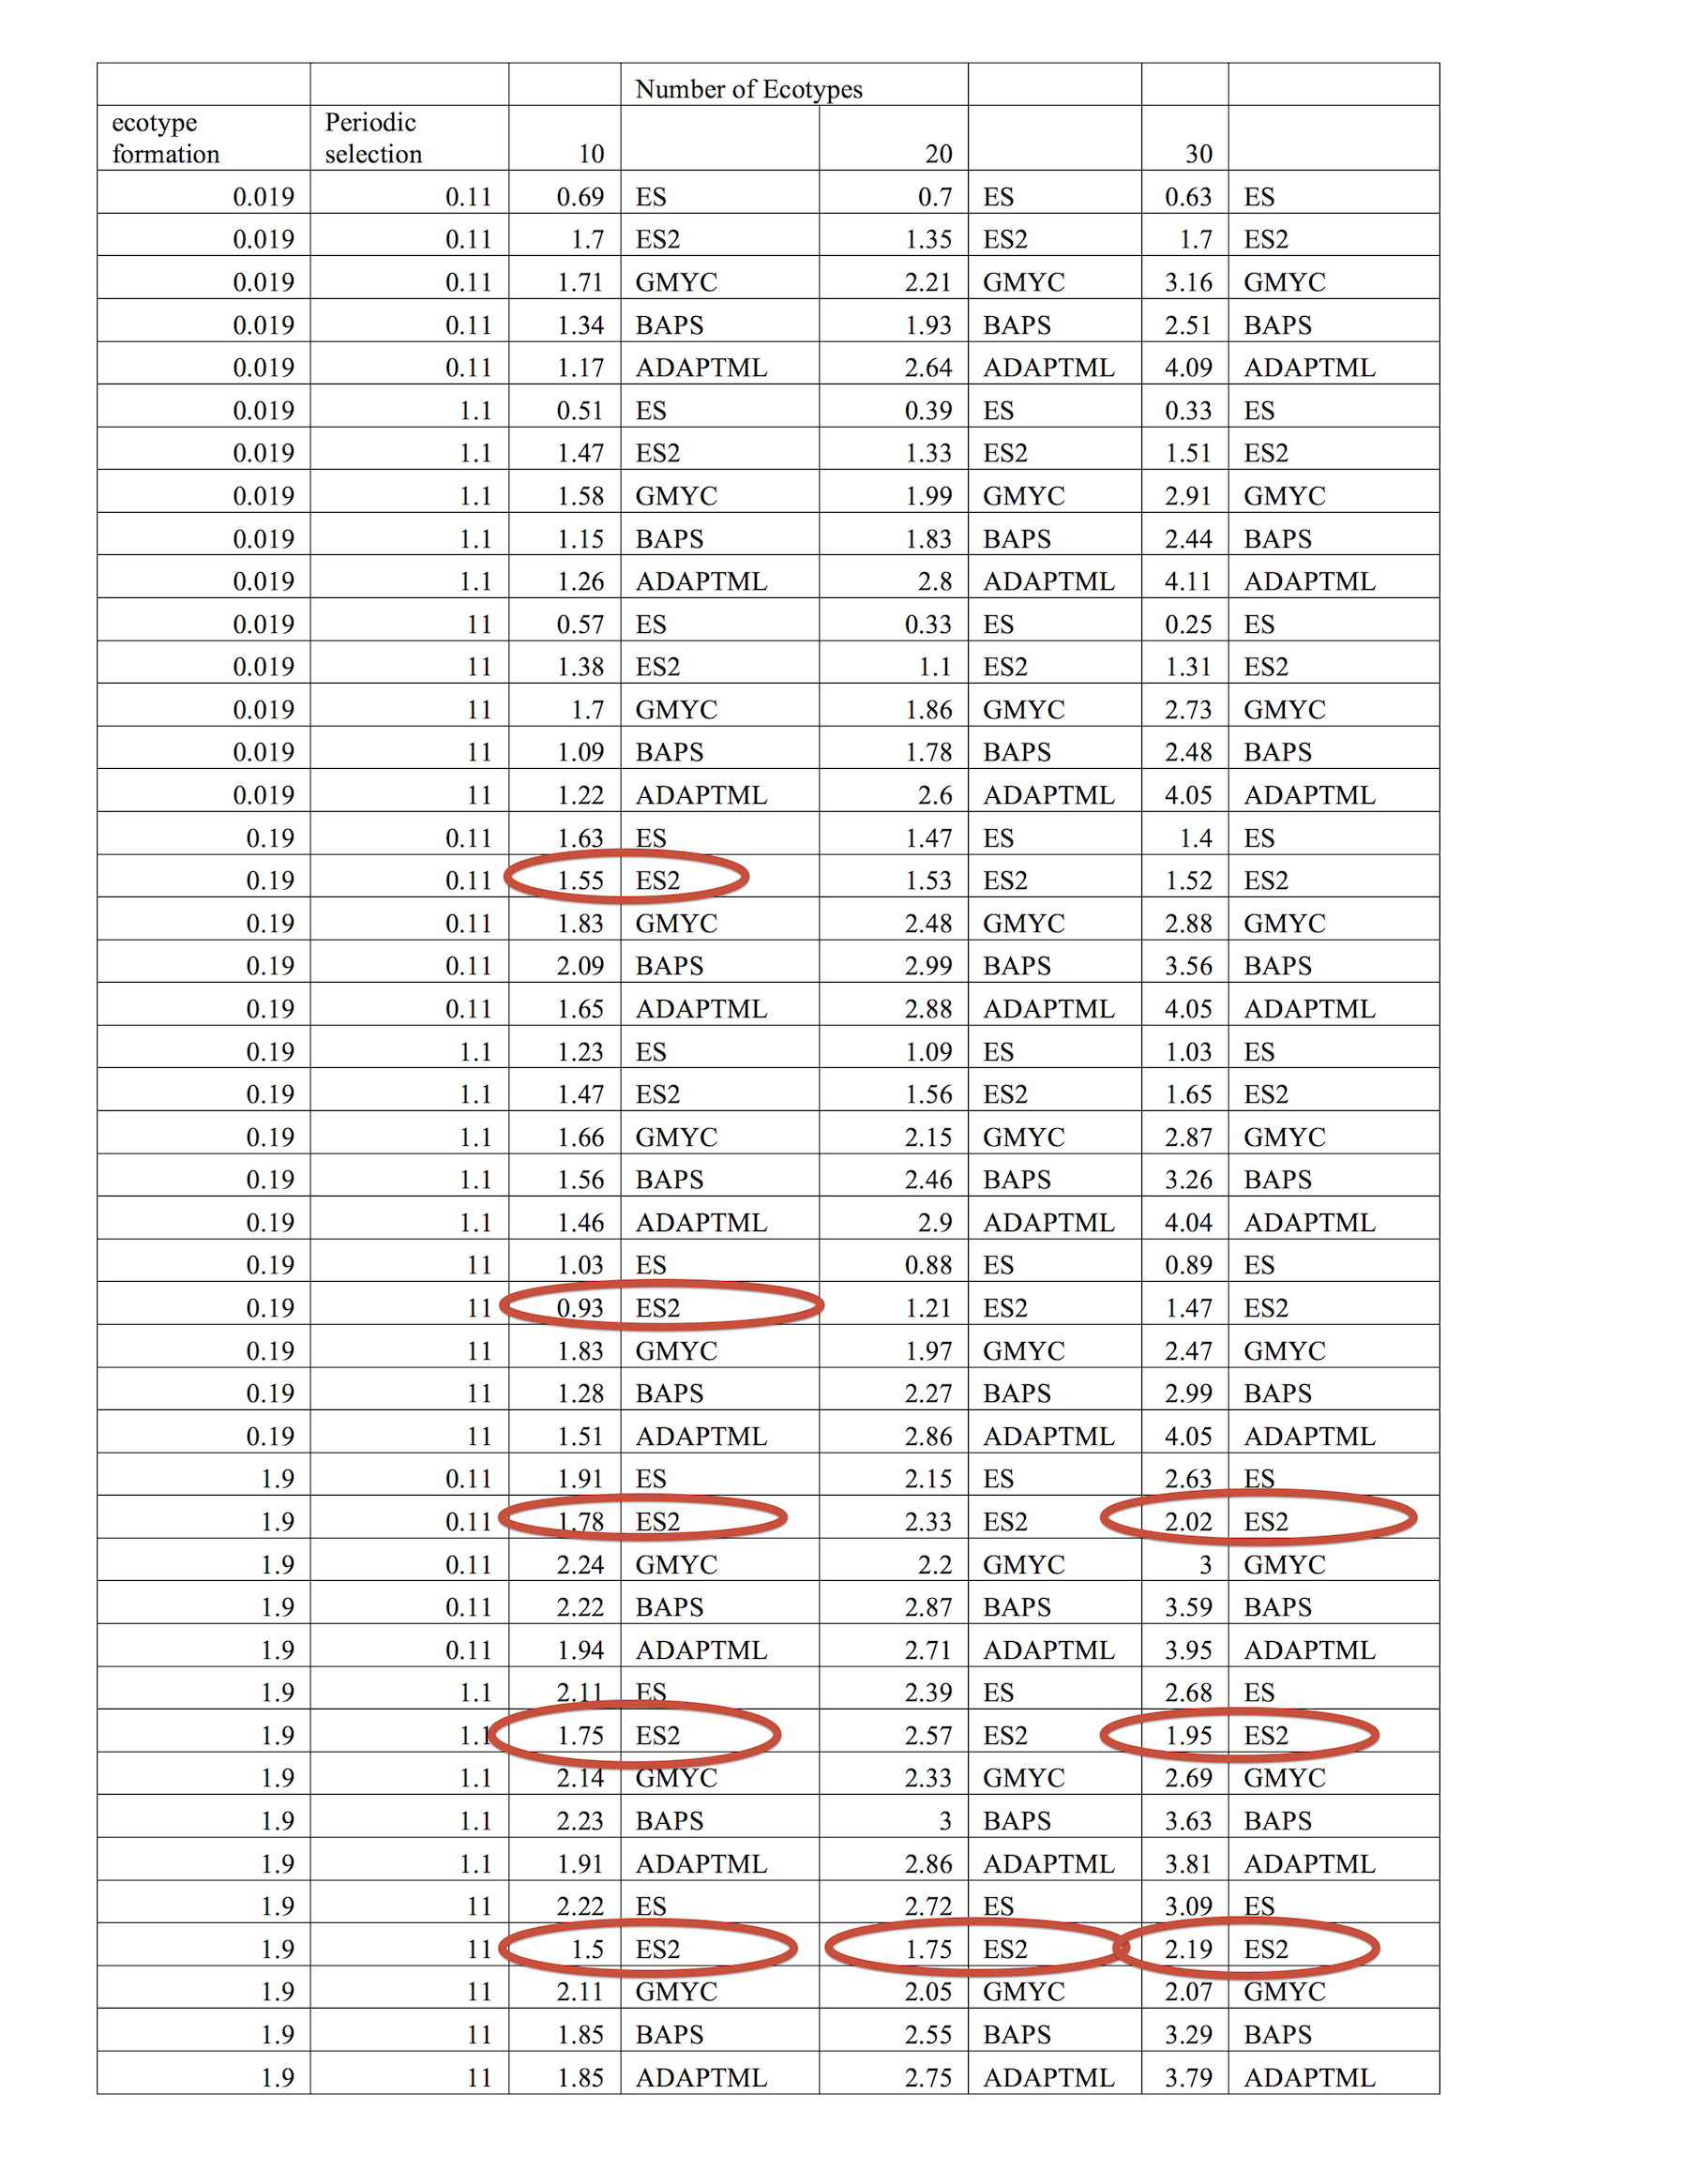
\includegraphics{images/ComparisonTable1.png}
    \label{fig:ComparisonSmall}
\end{figure}

\subsection*{Analysis of in silico-generated sequences}
The majority of my work was putting together a database of in silico generated sequences demarcation runs.
\subsubsection*{ES2 on smaller datasets}
\subsubsection*{All demarcation programs on large datasets}
\subsection*{\emph{Bacillus} sequences}
\subsection*{Running time}
\section{Chapter Summary}
In this chapter I discussed the motivation and thought process behind our experiments.
I gave a survey of other available demarcation programs (GMYC, BAPS, AdaptML, Random Demarcator), how we generated sample datasets, and described the metric used to compare the various outputs (Variation of Information metric).
I explain the choices behind which experiments we ran and finally sum up the important results received.






